\documentclass[12pt,a4]{article}




\usepackage{graphicx,amsmath,amssymb,amsthm, boxedminipage,xcolor}

%\usepackage[lined,boxed]{algorithm2e}

\usepackage{algorithm}
\usepackage{algpseudocode}

%\usepackage{algorithmic}
\usepackage{algpseudocode}
\usepackage{amsmath}
\usepackage{graphics}
\usepackage{epsfig}

\newtheorem{theorem}{Theorem}[section]
\newtheorem{proposition}[theorem]{Proposition}
\newtheorem{lemma}[theorem]{Lemma}
\newtheorem{corollary}[theorem]{Corollary}
\newtheorem{definition}[theorem]{Definition}

\newtheorem*{theorem*}{Theorem}
\newtheorem*{lemma*}{Lemma}
\newtheorem*{proposition*}{Proposition}


\newtheorem{exercise}[theorem]{Exercise}
\newtheorem{exerciseD}[theorem]{*Exercise}
\newtheorem{exerciseDD}[theorem]{**Exercise}

\let\oldexercise\exercise
\renewcommand{\exercise}{\oldexercise\normalfont}

%\let\oldexerciseD\exerciseD
%\renewcommand{\exerciseD}{\oldexerciseD\normalfont}

%\let\oldexerciseDD\exerciseDD
%\renewcommand{\exerciseDD}{\oldexerciseDD\normalfont}

\newcommand{\E}{\mathbb{E}}
%\newcommand{\nth}[1]{#1^{\textsuperscript{th}}}
\newcommand{\scalar}[2]{\ensuremath{\langle #1, #2\rangle}}
\newcommand{\floor}[1]{\left\lfloor #1 \right\rfloor}
\newcommand{\ceil}[1]{\left\lceil #1 \right\rceil}
\newcommand{\norm}[1]{\|#1\|}
\newcommand{\pfrac}[2]{\left(\frac{#1}{#2}\right)}
\newcommand{\nth}[1]{#1^{\textsuperscript{th}}}
\newcommand{\core}{\textnormal{core}}



\newif\ifsolution

\solutionfalse

\newcommand{\answer}[1]{
\ifsolution
{\color{blue} #1}
\else
\fi
}



\newcommand{\poly}{\textnormal{poly}}
\newcommand{\quasipol}{\textnormal{quasipol}}
\newcommand{\ssubexp}{\textnormal{stronglySubExp}}
\newcommand{\wsubexp}{\textnormal{weaklySubExp}}
\newcommand{\simplyexp}{\textnormal{E}}
\newcommand{\expo}{\textnormal{Exp}}



\newcommand{\N}{\mathbb{N}}
\newcommand{\nn}{\mathbb{N}_0^n}
\newcommand{\R}{\mathbb{R}}
\newcommand{\Z}{\mathbb{Z}}


\definecolor{darkgreen}{rgb}{0,0.6,0}


\date{}

\title{
  Mathematical Foundations \\of \\Computer Science\\
  \vspace{3mm}
{\normalsize CS 499,	Shanghai Jiaotong University,  Dominik Scheder}
}

\begin{document}

\maketitle

%\begin{quotation}
%  You are welcome to discuss the exercises in the discussion
%  forum. Please take them serious. Doing the exercises is as important
%  than watching the videos.
%
%  I intentionally included very challenging exercises and marked them
%  with one or two ``$*$''. No star means you should be able to solve
%  the exercises without big problems once you have understood
%  the material from the video lecture. One star means it requires 
%  significant additional thinking. Two stars means it is not 
%  unlikely that you will fail to solve them, even once you have understood
%  the material and thought a lot about the exercise. Don't feel bad
%  if you fail. Failure is part of learning.
%
%  This is the first time this course is online. Thus there might be mistakes
%  (typos or more serious conceptual mistakes) in the exercises. I will be 
%  grateful if you point them out to me!
%\end{quotation}





\setcounter{section}{9}

\section{Network Flow}



\begin{itemize}
 \item Homework assignment published on Monday 2018-05-07
 \item Submit questions and first solution by Sunday, 2018-05-13, 12:00
 \item Submit final solution by Sunday, 2018-05-20.
\end{itemize}



\begin{exercise}[From the video lecture]
   Recall the definition of the value of a flow: ${\rm val}(f) = \sum_{v \in V} f(s,v)$.
   Let $S \subseteq V$ be a set of vertices that contains $s$ but not $t$. Show that
   \begin{align*}
         {\rm val}(f) = \sum_{u \in S, v \in V \setminus S} f(u,v) \ .
   \end{align*}
   That is, the total amount of flow leaving $s$ equals the total amount of flow 
   going from $S$ to $V \setminus S$.
   \textbf{Remark.} It sounds obvious. However, find a formal proof that works with the 
   axiomatic definition of flows. 
\end{exercise}

   \par \textbf{Proof.}
   \par First, we use $e$ to denote an edge, and it is obvious that for each $v\in V-{s,t}$:
   \begin{align*}
         \sum_{e\,into\,v} f(e)= \sum_{e\,out\,of\,v}f(e)\
   \end{align*}
   \par We call it flow conservation, and with the help of it we can know that:
   \begin{align*}
         {\rm val}(f)
         =\sum_{e\,out\,of\,s} f(e)
         =\sum_{v\in S}(\sum_{e\,out\,of\,u}f(e)-\sum_{e\,into\,v}f(e))
         =\sum_{e\,out\,of\,A}f(e)-\sum_{e\,into\,A}f(e)
          \
   \end{align*}
   \par As for the flow, if it is from $S$ to $V-S$, it is a positive one, otherwise it is a negative one. Namely, the formula above it is
   \begin{align*}
         \sum_{u \in S, v \in V \setminus S} f(u,v) \
   \end{align*}



\begin{exercise}
Let $G = (V,E,c)$ be a flow network.
  Prove that flow is ``transitive'' in the following sense: 
  If there is a flow from $s$ to $r$ of value $k$,
  and a flow from $r$ to $t$ of value $k$, then
  there is a flow from $s$ to $t$ of value $k$.
  \textbf{Hint.} The solution is extremely short. If you are trying
  something that needs more than 3 lines to write, you are on the wrong
  track.
\end{exercise}

  \par\textbf{Proof.}
  \par We use the water to embody the flow. If the water from $s$ to $r$ of value $k$ is exactly that $r$ to $t$, then obviously the statement holds. If there is some not flowing to $t$ but to some other vertex, from the flow conservation we can know there must be some water flow into $r$ with the same quantity, so there is also a flow from $s$ to $t$.




\subsection{An Algorithm for Maximum Flow}

Recall the algorithm for Maximum Flow presented in the video. It is usually called
the Ford-Fulkerson method.

\begin{algorithm}[h]
\caption{Ford-Fulkerson Method}\label{algorithm-encoding}
\begin{algorithmic}[1]
\Procedure{FF}{$G=(V, E), s, t, c$} 
  \State Initialize $f$ to be the all-$0$-flow.
   \While{there is a path $p$ form $s$ to $t$ in the residual network $G_{f}$}
    \State $c_{\rm min} := \min \{ c_f(e) \ | \ e \in p \}$ 
    \State let $f_p$ be the flow in $G_f$ that routes $c_{\rm min}$ flow along $p$
    \State $f:= f + f_p$
   \EndWhile
   \State \texttt{//} now $f$ is a maximum flow
  \State $S := \{v \in V \ | \ G_f \textnormal{ contains a path from } s \textnormal{ to } v \}$
  \State \texttt{//} $S$ is a minimum cut
  \State \Return $(f,S)$
\EndProcedure
\end{algorithmic}
\end{algorithm}

We proved in the lecture that $f$ is a maximum flow and $S$ is a minimum cut,
by showing that upon termination of the while-loop, ${\rm val}(f) = {\rm cap}(S)$.
The problem is that the while-loop might not terminate. In fact, there is an example
with capacities in $\mathbb{R}$ for which the while loop does not terminate, and the 
value of $f$ does not even converge to the value of a maximum flow. As indicated
in the video, a little twist fixes this:
\begin{quotation}
  \textbf{Edmonds-Karp Algorithm:} Execute the above 
  Ford-Fulkerson Method, but in every iteration choose $p$ to be a 
  shortest $s$-$t$-path in $G_f$. Here, ``shortest'' means minimum number of edges.
\end{quotation}
In a series of exercises, you will now show that this algorithm always terminates
after at most $n \cdot m$ iterations of the while loop (here $n = |V|$ and $m = |E|$).

\begin{definition}
   Let $(G,s,t,c)$ be a flow network and $k \in \mathbb{N}_0$.
   A {\em $k$-layering} is a partition of $V = V_0 \cup \dots \cup V_k$ such that
   (1) $s \in V_0$, (2) $t \in V_k$, (3)
   for every edge $(u,v) \in E$ the following holds: suppose $u \in V_i$ and $v \in V_j$.
   Then $j \leq i+1$. 
   In words, point (3) states that every edge moves at most one level forward.
\end{definition}

The figure below illustrates this concept: for one network we show two possible layerings
and something that looks like a layering but is not:
\begin{center}
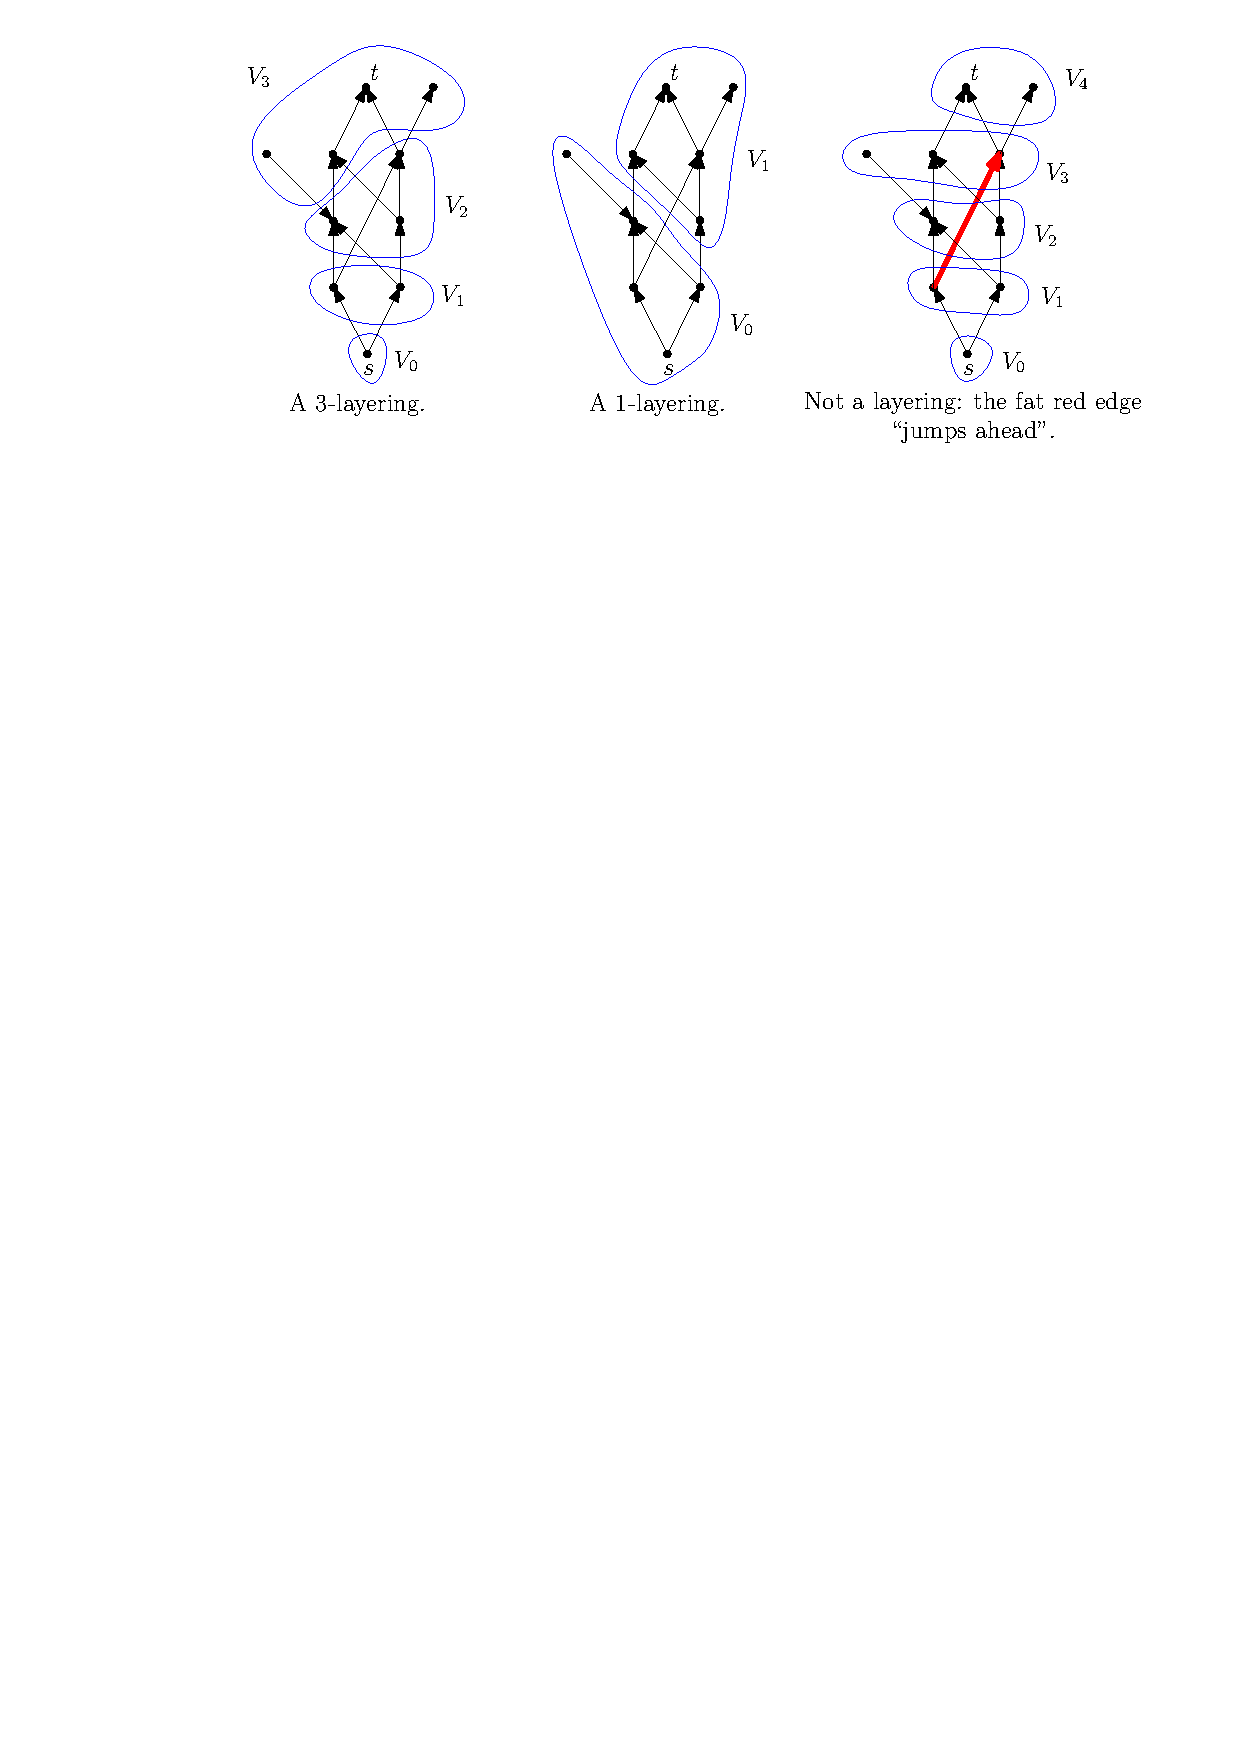
\includegraphics[width=\textwidth]{figures/layering.pdf}
\end{center}


\begin{exercise}
   Suppose the network $(G,s,t,c)$ has a $k$-layering. Show that ${\rm dist}(s,t) \geq k$.
   That is, every $s$-$t$-path in $G$ has at most $k$ edges.
\end{exercise}

\begin{exercise}
   Conversely, suppose ${\rm dist}(s,t) = k$. Show that $(G,s,t,c)$ has a $k$-layering.
\end{exercise}



Let $(G,s,t,c)$ be a flow network and $V_0,\dots,V_k$ a $k$-layering. We call this 
layering {\em optimal} if ${\rm dist}_G(s,t) = k$. Here, ${\rm dist}_G(u,v)$ 
is the shortest-path distance from $s$ to $t$ (measured by number of edges).
If there is no path from $s$ to $t$, we set ${\rm dist}_G(s,t) = \infty$. In this case, 
no layering is optimal.
For example, the $3$-layering
in the above figure is optimal, but the $1$-layering in the middle of the above figure
is not.
Let us explore how layerings and the Ford-Fulkerson Method interact.


\begin{exercise}
   Let $(G,s,t,c)$ be a flow network and $V_0, V_1, \dots, V_k$ be an optimal layering
   (that is, $k = {\rm dist}_G(s,t)$.
   Let $p$ be a path from $s$ to $t$ of length $k$. 
   Suppose we route some flow $f$ along $p$ (of some
   value $c_{\rm min} > 0$) and let $(G_f,s,t,c_f)$ be the residual network. Show that
   $V_0, V_1,\dots, V_k$ is a layering of $(G_f,s,t,c_f)$, too. Obviously, condition (1) and (2) in
   the definition of $k$-layerings still hold, so you only have to check  condition (3).
\end{exercise}

\textbf{Solution}

For any edge $(u,v)$ in path $p$ in $G$, $u \in V_i$, $v \in V_j$, $j \leq i + 1$.

Since the length of the path is $k$, $j = i + 1$

In the residual graph $G_f$, $(u,v)$ split to $(u,v)$ and $(v,u)$.

Obviously, $(u,v)$ still satisfies the condition (3).

For $(v,u)$, $i = j-1 \leq j+1$, thus it satisfies the condition (3), too.

Therefore, $V_0, V_1, \dots, V_k$ is a layering of $(G_f, s, t, c_f)$, too.


\begin{exercise}
   Show that every network $(G,s,t,c)$ has an optimal layering, provided there is a path
   from $s$ to $t$.
\end{exercise}

\textbf{Solution}

\textbf{Case 1}: When the provided path from $s$ to $t$ is the shortest-path with length $k$, according to \textbf{Exercies 10.5}, there is a $k$-layering. Thus, the network has an optimal layering.

\textbf{Case 2}: When the provided path from $s$ to $t$ is not the shortest-path, then there is another shortest-path from $s$ to $t$ with length $k$. According to \textbf{Exercies 10.5}, there is a $k$-layering. Thus, the network has an optimal layering.


\begin{exercise}
   Imagine we are in some iteration of the while-loop of the Ford-Fulkerson method.
   Let $V_0, \dots, V_k$ be an optimal layering of $(G,s,t,c)$. Show that after at most $m$
   iterations of the while-loop, $V_0,\dots,V_k$ ceases
   to be an optimal layering. \textbf{Remark.} Note that it is the {\em network} that changes from
   iteration to iteration of the while-loop, not the partition $V_0,\dots,V_k$. We consider
   the partition $V_0,\dots,V_k$ to be fixed in this exercise.
\end{exercise}

\textbf{Solution}

After every iteration, an edge is completely reversed. Note that the reversed edge cannot appear in the shortest path again becauce it "goes back" to lower layer.

When the edge $(u,v)$ is reversed to $(v,u)$, the chosen path $s \rightarrow \dots u \rightarrow v \rightarrow \dots t$ no longer exists. And the algorithm choose the shortest path, so the chosen path is the shortest path and the reversed edge is part of the shortest path, namely the edge crossing the layers. There may be many shortest paths. And there are at most $m$ edges crossing the layers, so after at most $m$ iterations, all the edges of the original shortest paths is reversed and the new shortest paths have a longer length. So $V_0, V_1, \dots, V_n$ ceases to be an optimal layering.



\begin{exercise}
Show that the Edmonds-Karp algorithm terminates after $n \cdot m$ iterations of the 
while-loop. \textbf{Hint.} Initially, compute an optimal $k$-layering (which?). Then keep
this layering as long as its optimal. Once it ceases to be optimal, compute a new optimal
layering. Note that the Edmonds-Karp algorithm does not actually need to compute any
layering. It's us who compute it to show that $n \cdot m$ bound on the number of iterations.
\end{exercise}

\begin{exercise}
   Show that every network has a maximum flow $f$. 
   That is, a flow $f$ such that ${\rm val}(f) \geq {\rm val}(f')$ for every flow $f'$.
   \textbf{Remark.} This sounds obvious but it is not. In fact, there might be an infinite
   sequence of flows $f_1, f_2, f_3, \dots$ of increasing value that does not reach any maximum.
    Use the previous exercises!
\end{exercise}



\end{document}
